\section{Numerical validation in the commuting Gaussian sector}
\label{sec:numerical}

This section validates the commuting Gaussian theory by direct finite-bath trace-out,
analytic prediction, and stochastic imaginary-time sampling for the \emph{same}
Hamiltonian parameters.

\subsection{Common model and exact reference}

We use a five-level system with
\begin{equation}
H_S=\sum_{i=0}^{4}E_i\lvert i\rangle\!\langle i\rvert,\qquad E_0=0,
\end{equation}
and projector coupling operator
\begin{equation}
P=\lvert 4\rangle\!\langle 4\rvert,\qquad P^2=P.
\end{equation}
The nonzero energies are sampled once from a seeded random draw and then held
fixed for the full parameter sweep (exact values and seed are listed in
Appendix~\ref{app:numerics_implementation}). The bosonic bath and coupling are
\begin{align}
H_B &= \sum_k\omega_k\!\left(a_k^\dagger a_k+\tfrac12\right),\\
H_I &= P\otimes\sum_k c_k x_k,\qquad
x_k=\frac{a_k+a_k^\dagger}{\sqrt{2\omega_k}}.
\end{align}
No counterterm is included, so the renormalization is explicitly visible in
the reduced state. The exact benchmark at each parameter point is
\begin{equation}
\rho_S^{\mathrm{ED}}(\beta)
=
\frac{\Tr_B[e^{-\beta H_{\mathrm{tot}}}]}{\Tr[e^{-\beta H_{\mathrm{tot}}}]},
\label{eq:rho_ed_definition}
\end{equation}
computed by exact diagonalization with increasing bosonic cutoff to verify
convergence.

The continuum target spectrum is Ohmic with exponential cutoff,
\begin{equation}
J_g(\omega)=2\eta g^2\,\omega\,e^{-\omega/\omega_c},
\end{equation}
and is discretized into a finite mode set used in ED and in stochastic sampling.
Implementation details of the mode discretization and random-seed conventions
are given in Appendix~\ref{app:numerics_implementation}.
The discretized and continuum renormalization scales are
\begin{equation}
\lambda_{\mathrm{disc}}
=
\sum_k\frac{c_k^2}{2\omega_k^2},
\qquad
\lambda_{\mathrm{cont}}
=
\frac{1}{\pi}\int_0^\infty\frac{J_g(\omega)}{\omega}\,d\omega
\propto g^2.
\label{eq:lambda_defs}
\end{equation}

In the commuting Gaussian case the predicted mean-force Hamiltonian is
\begin{equation}
H_{\mathrm{MF}}=H_S-\lambda P+\mathrm{const},
\label{eq:hmf_projector_form}
\end{equation}
hence
\begin{equation}
\rho_S^{\mathrm{pred}}(\beta)\propto e^{-\beta(H_S-\lambda_{\mathrm{disc}}P)}.
\end{equation}

\subsection{LT-CG-1: beta sweep (ED, analytic, HS-path, HS-scalar)}

\paragraph*{Implementation.}
For each $(\beta,g)$ point we compute:
\begin{enumerate}
\item exact trace-out state $\rho_S^{\mathrm{ED}}$ from Eq.~\eqref{eq:rho_ed_definition},
\item analytic commuting state $\rho_S^{\mathrm{pred}}$,
\item HS-path estimate: sample a Gaussian field $\xi(\tau_j)$ on an imaginary-time
grid from the kernel covariance and evaluate
$X\approx\Delta\tau\sum_j\xi(\tau_j)$,
\item HS-scalar estimate: sample $X\sim\mathcal N(0,C_\beta)$ directly with
$C_\beta=2\beta\lambda_{\mathrm{disc}}$.
\end{enumerate}
All reported states are explicitly renormalized to unit trace before extracting
observables.

\paragraph*{Plotted observables.}
Panel (A) plots $p_4(\beta)=\langle 4|\rho_S|4\rangle$ for all four methods.
Panel (B) plots
\begin{equation}
\lambda_{\mathrm{est}}
=
E_4-E_0+\frac{1}{\beta}\log\!\left(\frac{p_4}{p_0}\right),
\label{eq:lambda_est}
\end{equation}
as $\lambda_{\mathrm{est}}/g^2$ vs $\beta$, together with
$\lambda_{\mathrm{disc}}/g^2$ and $\lambda_{\mathrm{cont}}/g^2$.
Panel (C) shows the individual populations $p_i$ at a representative
$(\beta,g)$ point for bare Gibbs, analytic HMF, and ED.
Panel (D) resolves the level-wise effective shift extracted from populations,
\begin{equation}
\Delta_i
=
E_i-E_0+\frac{1}{\beta}\log\!\left(\frac{p_i}{p_0}\right).
\label{eq:delta_i_est}
\end{equation}
For the projector-coupled model, the prediction is $\Delta_i=0$ for $i\neq 4$
and $\Delta_4=\lambda$.

\paragraph*{Physical claim tested.}
Agreement in panel (A) validates that ED trace-out, analytic commuting HMF, and
both stochastic implementations produce the same equilibrium populations.
Panel (B) tests the nontrivial scaling claim: the bath effect is a pure $g^2$
projector renormalization. Panels (C)-(D) show that the operator-level change is
localized to the coupled projector sector, while agreement with ED is maintained.

\begin{figure*}[t]
    \centering
    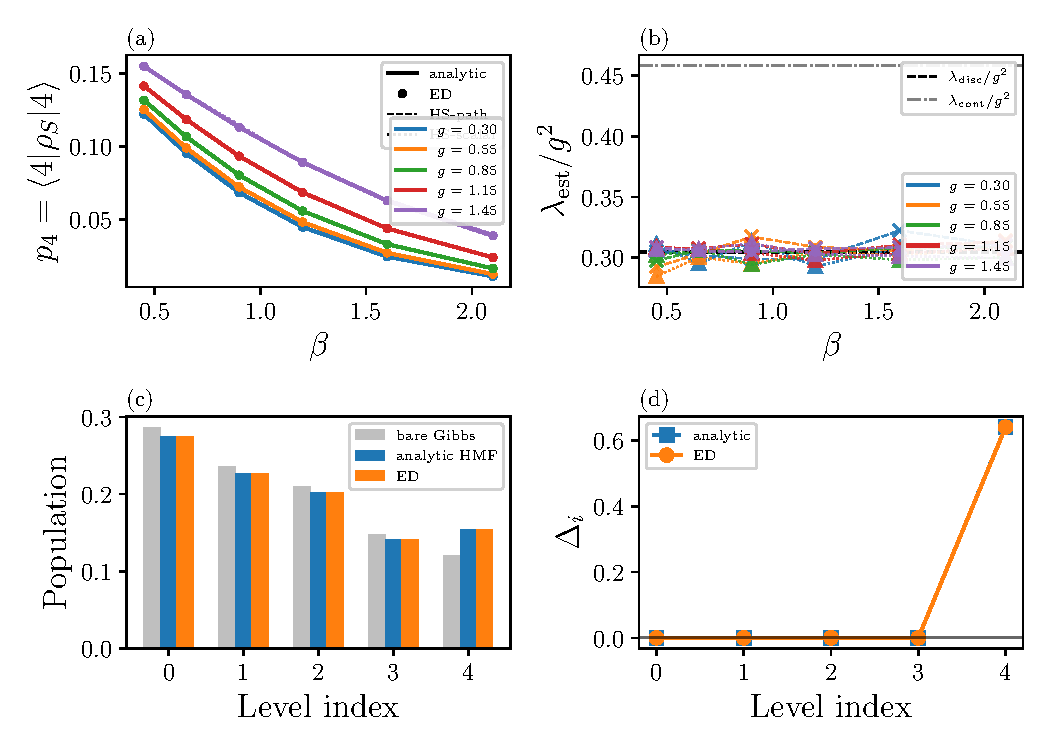
\includegraphics[width=\textwidth]{lt_cg_1.pdf}
    \caption{\label{fig:lt_cg_1}
    \textbf{LT-CG-1.}
    (A) $p_4(\beta)$ from ED, analytic commuting prediction, HS-path, and HS-scalar
    for multiple couplings $g$.
    (B) $\lambda_{\mathrm{est}}/g^2$ vs $\beta$ with
    $\lambda_{\mathrm{disc}}/g^2$ and $\lambda_{\mathrm{cont}}/g^2$ references.
    (C) Individual populations $p_i$ for bare Gibbs, analytic HMF, and ED at a
    representative $(\beta,g)$.
    (D) Level-resolved shifts $\Delta_i$ extracted from populations, showing that
    only the coupled level acquires the renormalization shift.}
\end{figure*}

\subsection{LT-CG-2: strong-coupling projector dominance}

\paragraph*{Implementation.}
At fixed large $\beta$, we sweep to stronger coupling and compare
$\rho_S^{\mathrm{ED}}$ with $\rho_S^{\mathrm{pred}}$.
From ED we extract
$H_{\mathrm{MF}}^{\mathrm{ED}}=-(1/\beta)\log\rho_S^{\mathrm{ED}}$
and fit it in the basis $\{\mathbf 1,H_S,P\}$:
\begin{equation}
H_{\mathrm{MF}}^{\mathrm{ED}}\approx c_0\mathbf 1+a_{H_S}H_S+a_P P.
\end{equation}

\paragraph*{Plotted observables and claim.}
Panel (A) shows $p_4$ vs $g^2$ (ED and analytic).
Panel (B) shows $a_P$ and $-\lambda_{\mathrm{disc}}$ vs $g^2$
(with $a_{H_S}$ included as reference).
This tests whether strong-coupling behavior remains controlled by the projected
interaction term predicted by Eq.~\eqref{eq:hmf_projector_form}.

\begin{figure}[t]
    \centering
    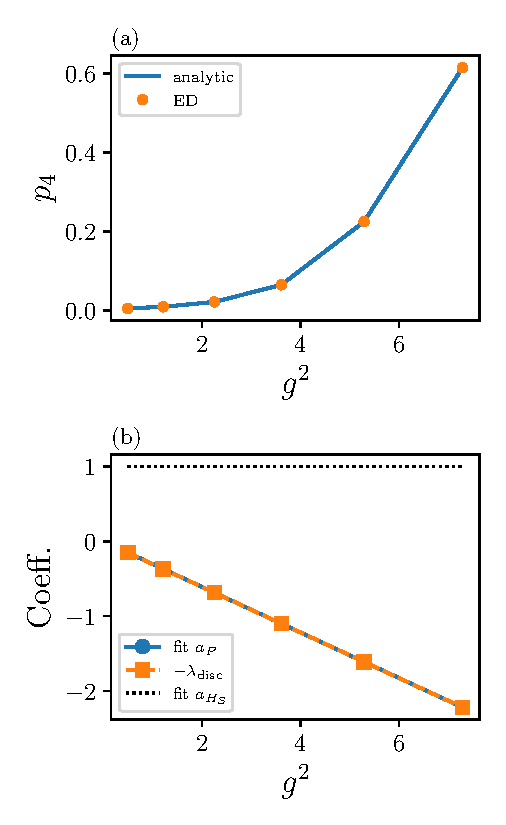
\includegraphics[width=\columnwidth]{lt_cg_2.pdf}
    \caption{\label{fig:lt_cg_2}
    \textbf{LT-CG-2.}
    (A) Strong-coupling crossover in $p_4$ vs $g^2$ (ED and analytic).
    (B) ED-extracted HMF coefficients in basis $\{\mathbf 1,H_S,P\}$,
    showing the projector coefficient tracking $-\lambda_{\mathrm{disc}}$.}
\end{figure}

Machine-readable metrics for both tests are stored in
the low-temperature simulation claim-metrics JSON output.
Full parameter tables and execution details are provided in the accompanying
simulation documentation and Appendix~\ref{app:numerics_implementation}.
